\documentclass[11pt]{article}
\usepackage{amsmath}
\usepackage[margin=.8in]{geometry}
\usepackage{enumitem}
\usepackage{float}
\usepackage{graphicx} % Required for inserting images
\usepackage{helvet}
\usepackage{hyperref}
\usepackage{listings}
\usepackage{mathptmx}
\usepackage{nameref}
\usepackage{pgfplots}
\usepackage{placeins}
\usepackage{subcaption}
\usepackage{titlesec}
\usepackage{wrapfig}
\renewcommand{\familydefault}{\sfdefault}
\graphicspath{{./images/}}
\titlespacing*{\section}{0pt}{0.1\baselineskip}{0.1\baselineskip}

\title{Complex Systems and Networks HW 2}
\author{Rachael Judy, Connor Klein, Josh Smith}
\date{31 March 2024}

\begin{document}
	\pgfplotsset{compat=1.18}
	\setlist[itemize]{noitemsep}
	\setlist[enumerate]{noitemsep}
	
	\maketitle
	
\section{Section 1: Random Policies and Social Recommendation Policy}\label{sec:q1}
\subsection{Simulation Description}\label{subsec:simulation}
% discuss hyperparameters like trials, epochs
This simulation uses variations on the Schelling model exploring Red and Green agents occupying a 2-dimensional LxL grid. This cellular automata can have Red squares, Green squares, or empty squares. The agents prefer to be near their own type and are fully happy if at k or more of the eight neighbors are of the same type. The simulation is designed with hyperparameters of a 40x40 (L=40) square grid with wraparound at the borders. The agents occupy 90\% ($\alpha=.9$) of the cells and k=3 neighbors are define happiness of the agent. The number of trials run for each case is set to 20 trials of 20 epochs each. Different relocation policies and their parameters are applied to determine where unhappy agents move to seek greater satisfaction.

\subsubsection{Happiness Function}
An agent is defined as completely happy if k or more of its neighbors are of the same group as itself. The partial happiness (happiness < 1) is defined as the number of neighbors of the same group over the total number of neighbors combined with a small bonus for adjacent empty spaces instead of adjacent mismatched neighbors. This can be expressed as $H(A_i) = \text{count}(N_i) + .25 \text{count}(N_e)$ where H is the happiness of an agent A of type i and $N_i$ is a neighbor of type i and $N_e$ is an adjacent empty square.

\subsubsection{Performance Metric}
The performance metric was selected to simply be the sum of the happiness of every agent in the cellular automata ie $\sum\limits_{a \in A} H(a)$.

\subsection{Policies}\label{subsec:policies}
The agent will consider moving only if it is unhappy. The basic policies modeled as described in the homework were a random move policy and a social network recommendation. The random move policy has a single parameter $q$ which limits how many random empty cells to visit looking for a cell where the agent will be happier than it is currently. 

The social network recommendation (SNR) will take a randomly selected set of n friends for each agent who will look in a pxp square around themselves and report suitable squares found. The agent than randomly selects one of the suitable squares and moves there. If none is available, it defaults to the random move policy. This policy was run over parameter values of p=[3,5] and n=[5, 10, 20].

\subsection{Results}
% for insertion of before/after plots
	\begin{figure}[h]
		\centering
		\begin{subfigure}{0.14\textwidth}
			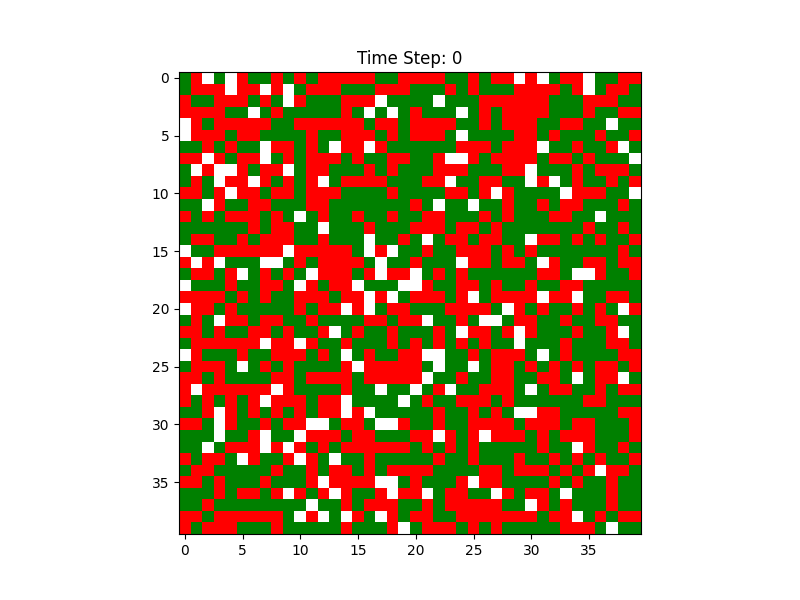
\includegraphics[width=\linewidth]{initial_random.png}
			\caption{\centering Random move}
		\end{subfigure}\hfill
		\begin{subfigure}{0.14\textwidth}
			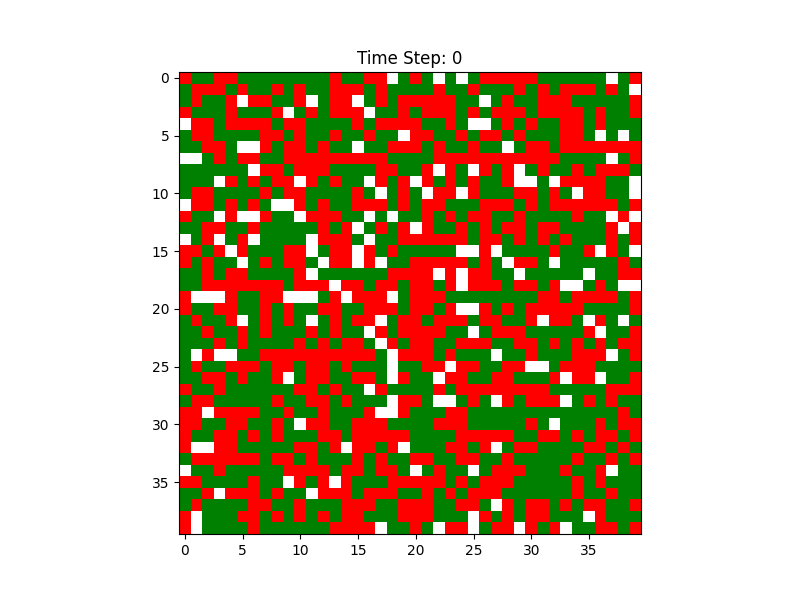
\includegraphics[width=\linewidth]{initial_social_n5p3.png}
			\caption{\centering SNR n=5, p=3}
		\end{subfigure}\hfill
		\begin{subfigure}{0.14\textwidth}
			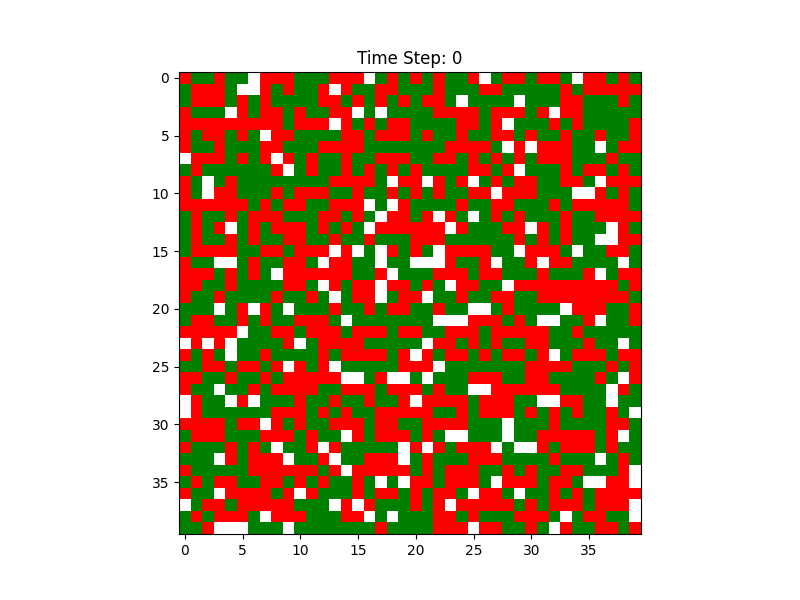
\includegraphics[width=\linewidth]{initial_social_n5p5.png}
			\caption{\centering SNR with n=5, p=5}
		\end{subfigure}\hfill
		\begin{subfigure}{0.14\textwidth}
			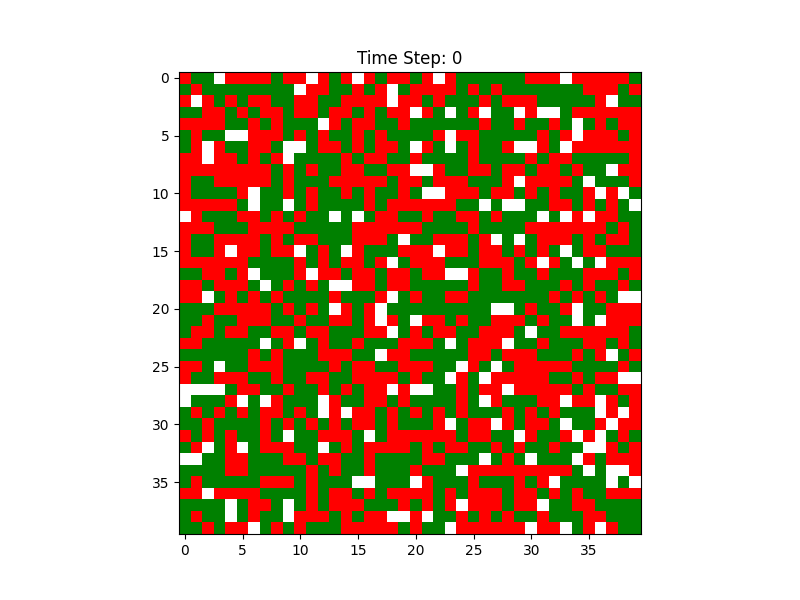
\includegraphics[width=\linewidth]{initial_social_n10p3.png}
			\caption{\centering SNR with n=10, p=3}
		\end{subfigure}\hfill
		\begin{subfigure}{0.14\textwidth}
			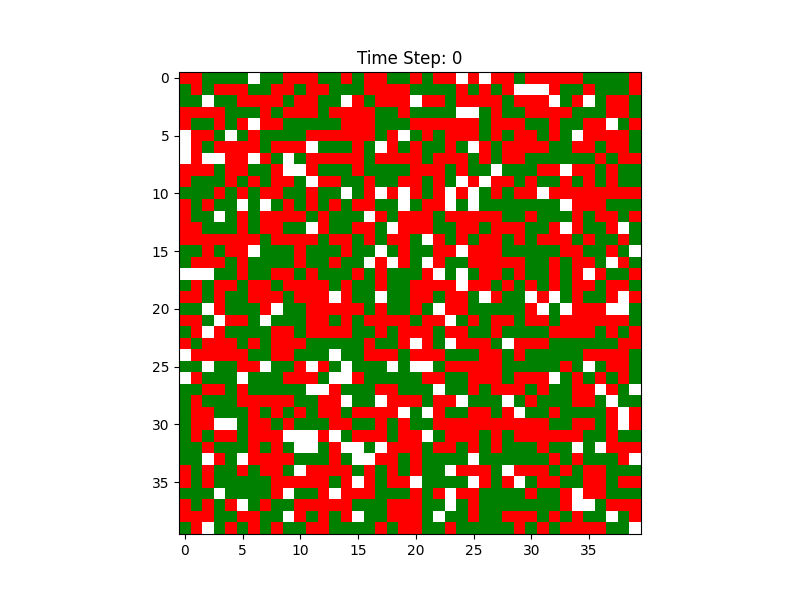
\includegraphics[width=\linewidth]{initial_social_n10p5.png}
			\caption{\centering SNR with n=10, p=5}
		\end{subfigure}\hfill
		\begin{subfigure}{0.14\textwidth}
			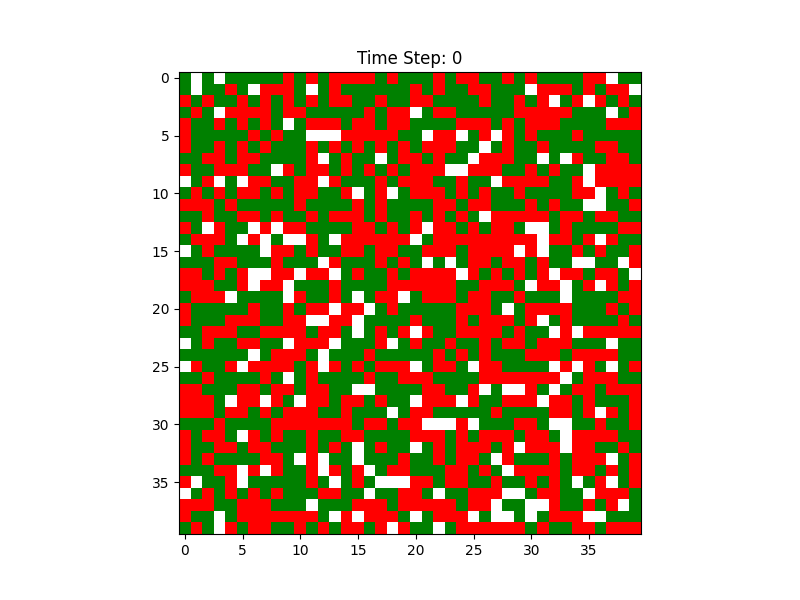
\includegraphics[width=\linewidth]{initial_social_n20p3.png}
			\caption{\centering SNR with n=20, p=3}
		\end{subfigure}\hfill
		\begin{subfigure}{0.14\textwidth}
			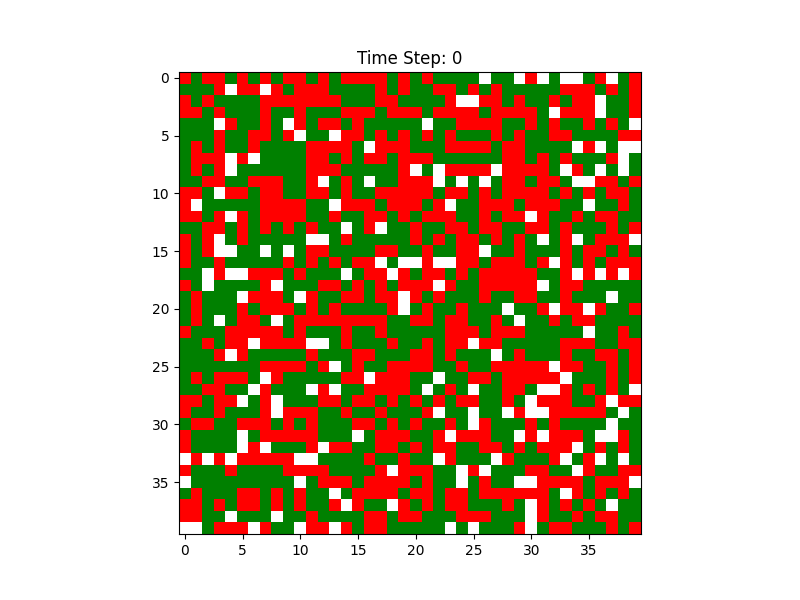
\includegraphics[width=\linewidth]{initial_social_n20p5.png}
			\caption{\centering SNR with n=20, p=5}
		\end{subfigure}
		\caption{Initial States}
	\end{figure}
	\begin{figure}[h]
		\centering
		\begin{subfigure}{0.14\textwidth}
			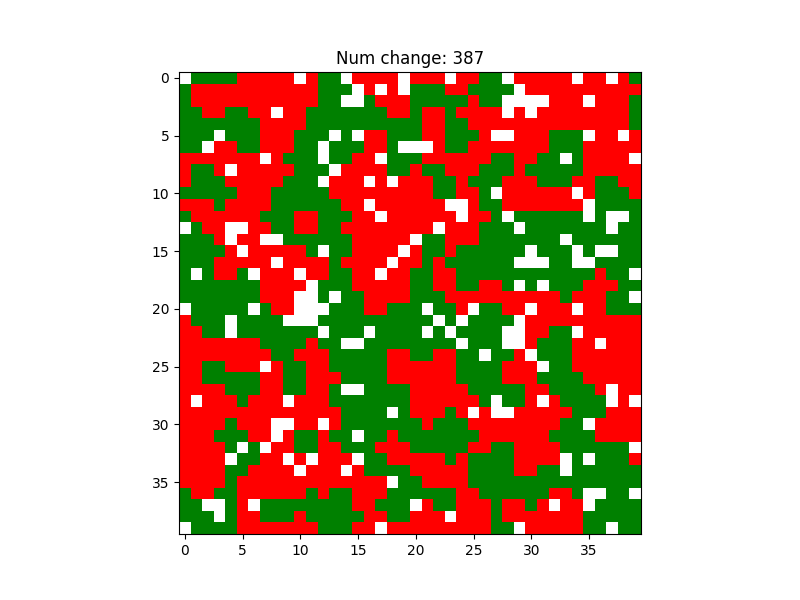
\includegraphics[width=\linewidth]{final_random.png}
			\caption{\centering Random move}
		\end{subfigure}\hfill
		\begin{subfigure}{0.14\textwidth}
			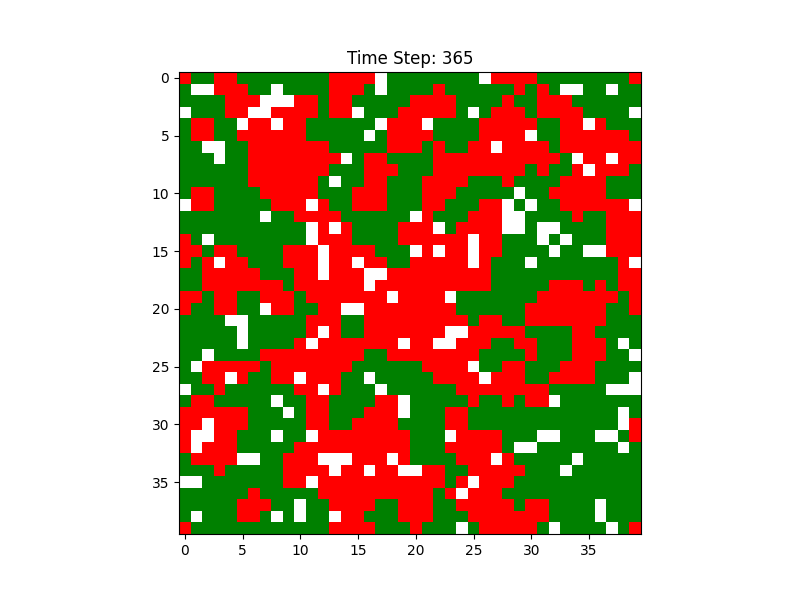
\includegraphics[width=\linewidth]{final_social_n5p3.png}
			\caption{\centering SNR with n=5, p=3}
		\end{subfigure}\hfill
		\begin{subfigure}{0.14\textwidth}
			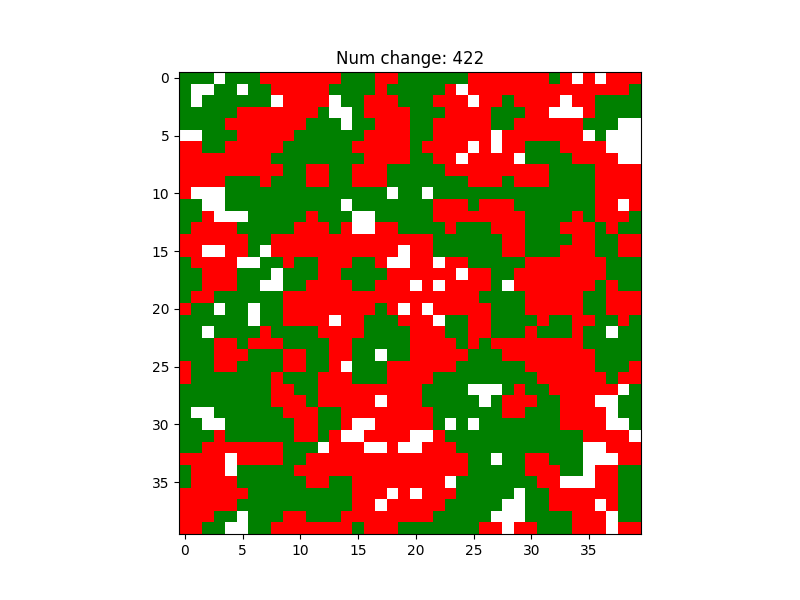
\includegraphics[width=\linewidth]{final_social_n5p5.png}
			\caption{\centering SNR with n=5, p=5}
		\end{subfigure}\hfill
		\begin{subfigure}{0.14\textwidth}
			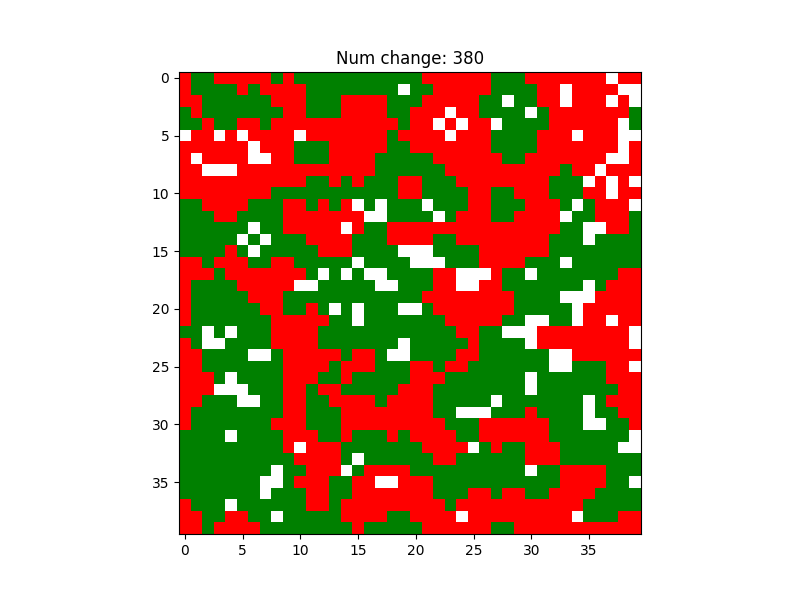
\includegraphics[width=\linewidth]{final_social_n10p3.png}
			\caption{\centering SNR with n=10, p=3}
		\end{subfigure}\hfill
		\begin{subfigure}{0.14\textwidth}
			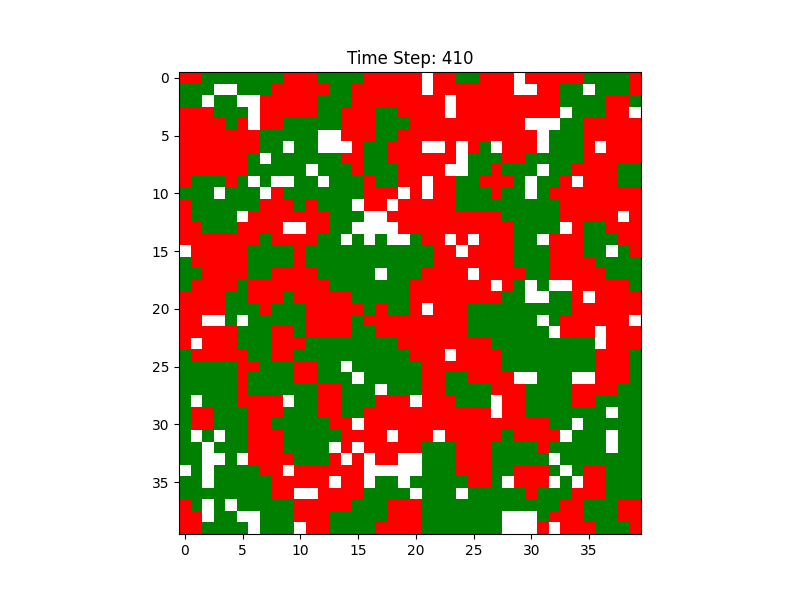
\includegraphics[width=\linewidth]{final_social_n10p5.png}
			\caption{\centering SNR with n=10, p=5}
		\end{subfigure}\hfill
		\begin{subfigure}{0.14\textwidth}
			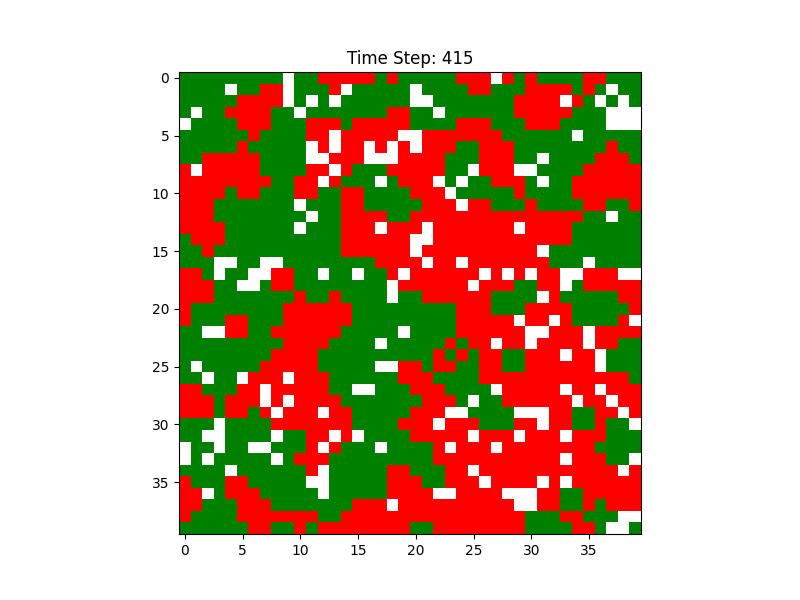
\includegraphics[width=\linewidth]{final_social_n20p3.png}
			\caption{\centering SNR with n=20, p=3}
		\end{subfigure}\hfill
		\begin{subfigure}{0.14\textwidth}
			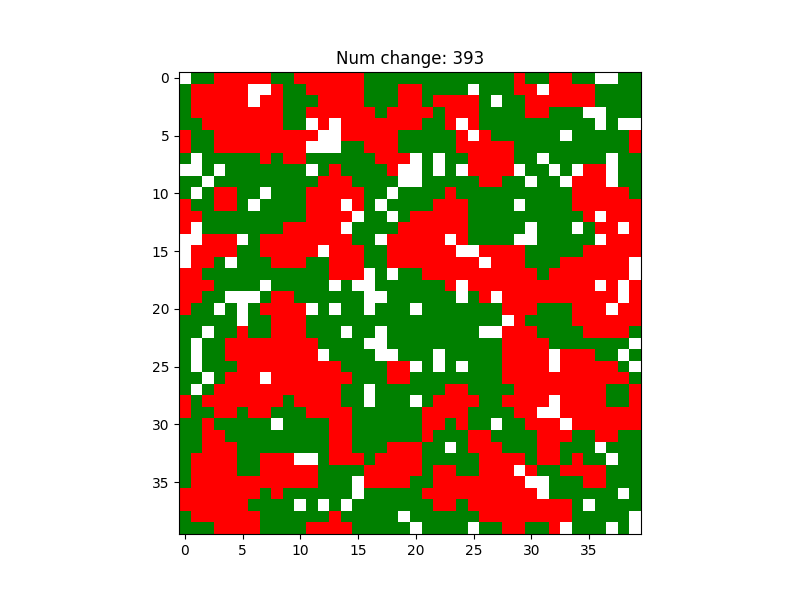
\includegraphics[width=\linewidth]{final_social_n20p5.png}
			\caption{\centering SNR with n=20, p=5}
		\end{subfigure}
		\caption{Final States of Random move and social network recommendation policies}
	\end{figure}

	\begin{figure}[h]
		\centering
		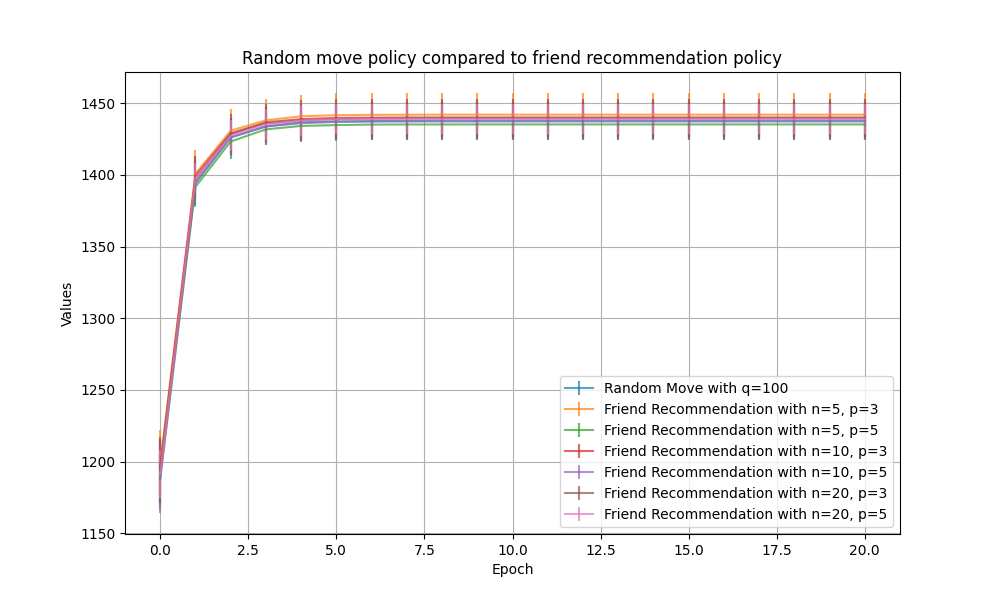
\includegraphics[width=\textwidth]{policies01.png}
		\caption{Time series comparing a random move policy with the network recommendation policy}
	\end{figure}
	\FloatBarrier

	\newpage
	\section{Section 2: Specialized Policies}
	\subsection{Rachael}
	\subsubsection{Policy Description}
	With the segregation in housing application of the Schelling Model, this idea can be expanded to include searching within one's own neighborhood (SN) for a better house in the same area. This policy has two parameters $w$ and $\beta$. The parameter $w$ defines the number of moves away from one's own cell that can be asked (a degree of separation sort of idea) and $\beta$ defines the probability that a neighbor who is not the same type as the searcher is asked for available spots. This simulates asking neighbors of the same type who ask neighbors of the same type for available spots. If none of the neighbors have a good spot, the random move policy is applied. This policy is implemented as a BFS from the agent along matching agents to the separation limit.
	
	\subsubsection{Results}
	% for insertion of before/after plots
	\begin{figure}[h]
		\centering
		\begin{subfigure}{0.14\textwidth}
			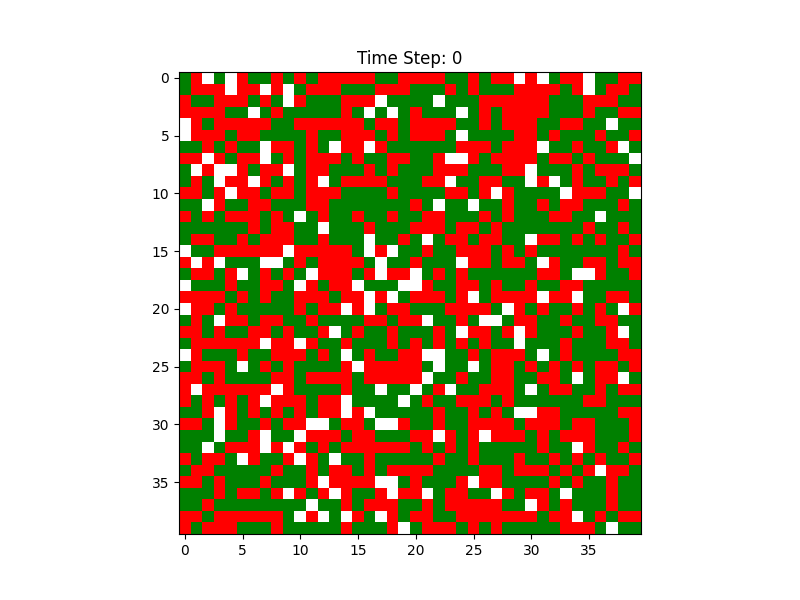
\includegraphics[width=\linewidth]{initial_random.png}
			\caption{\centering Random move}
		\end{subfigure}\hfill
		\begin{subfigure}{0.14\textwidth}
			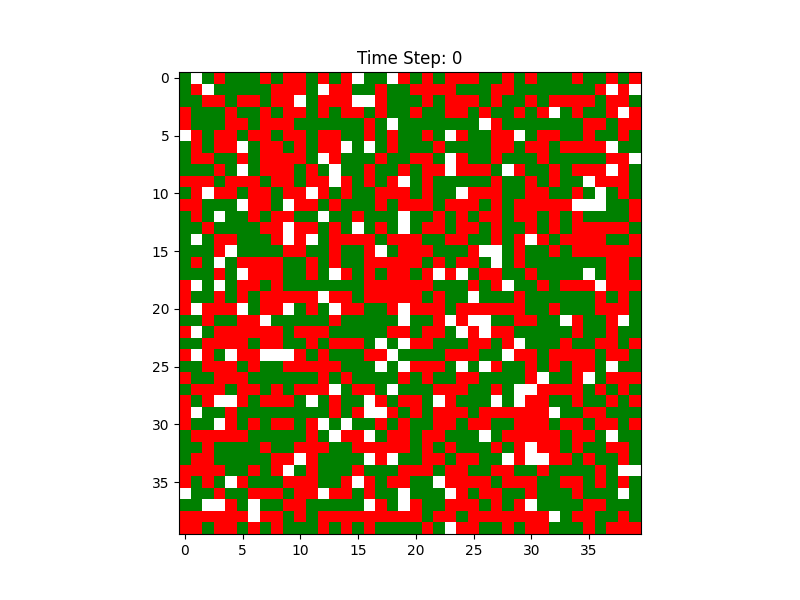
\includegraphics[width=\linewidth]{initial_cluster_w5b10.png}
			\caption{\centering SN w=5, beta=.1}
		\end{subfigure}\hfill
		\begin{subfigure}{0.14\textwidth}
			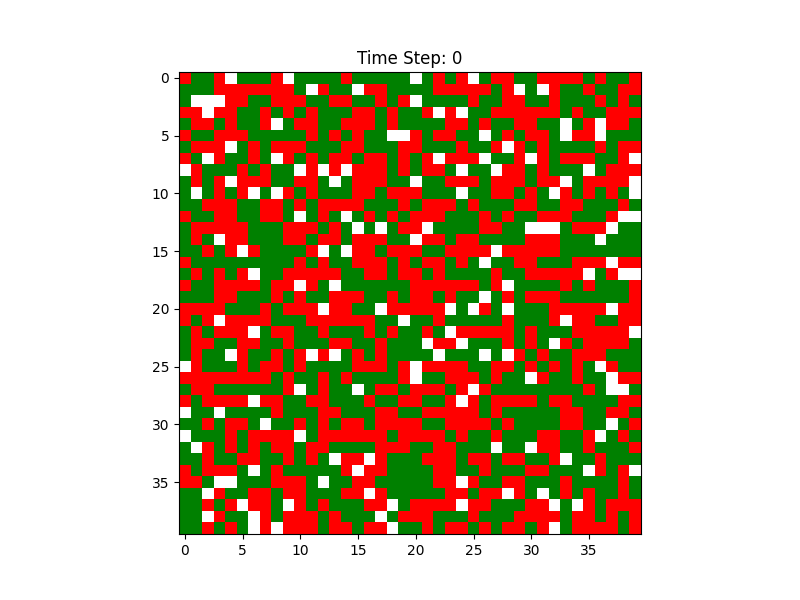
\includegraphics[width=\linewidth]{initial_cluster_w10b10.png}
			\caption{\centering SN w=10, beta=.1}
		\end{subfigure}\hfill
		\begin{subfigure}{0.14\textwidth}
			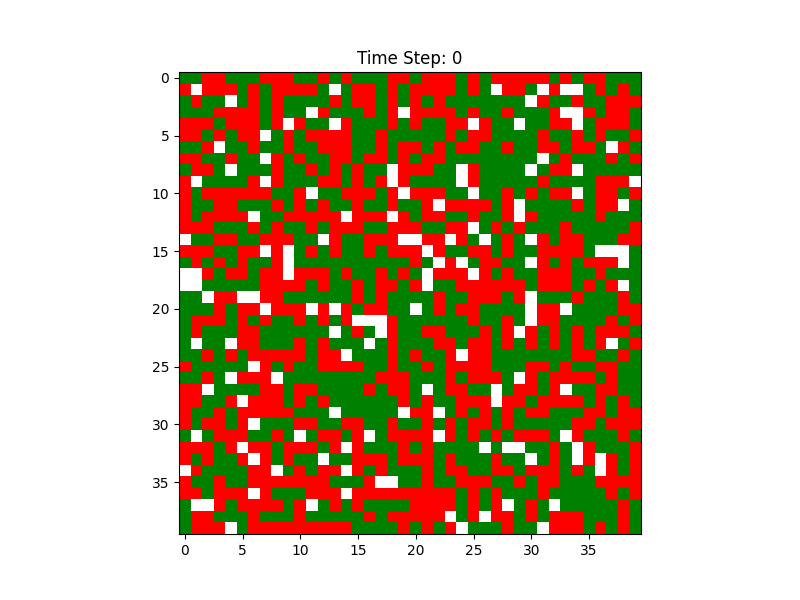
\includegraphics[width=\linewidth]{initial_cluster_w20b10.png}
			\caption{\centering SN w=20, beta=.1}
		\end{subfigure}\hfill
		\begin{subfigure}{0.14\textwidth}
			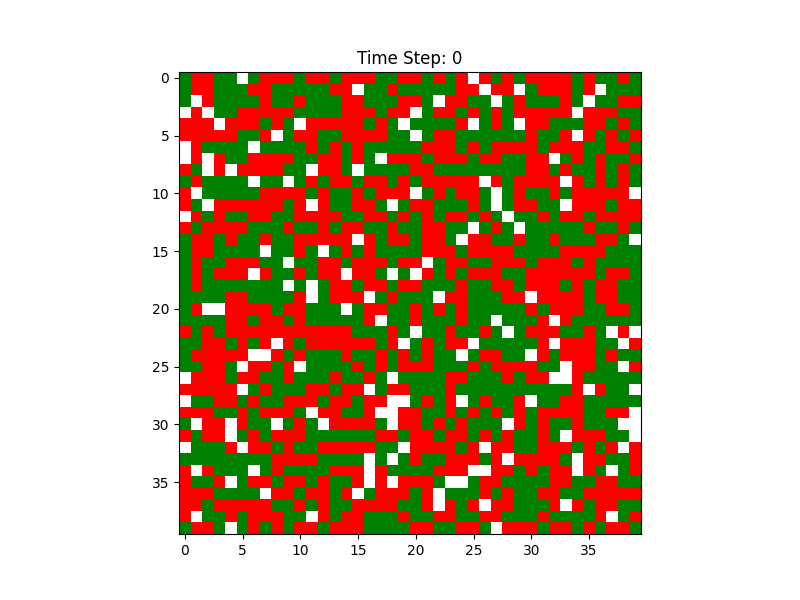
\includegraphics[width=\linewidth]{initial_cluster_w5b20.png}
			\caption{\centering SN w=5, beta=.2}
		\end{subfigure}\hfill
		\begin{subfigure}{0.14\textwidth}
			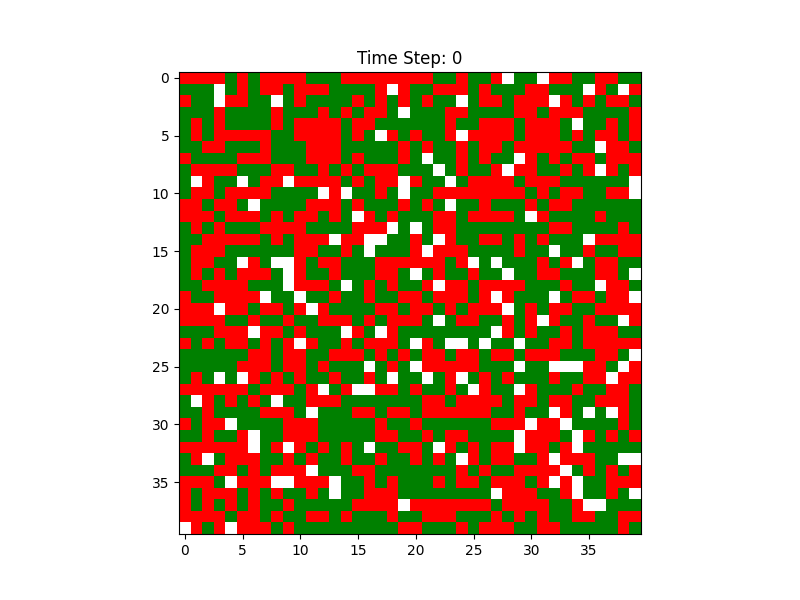
\includegraphics[width=\linewidth]{initial_cluster_w10b20.png}
			\caption{\centering SN w=10, beta=.2}
		\end{subfigure}\hfill
		\begin{subfigure}{0.14\textwidth}
			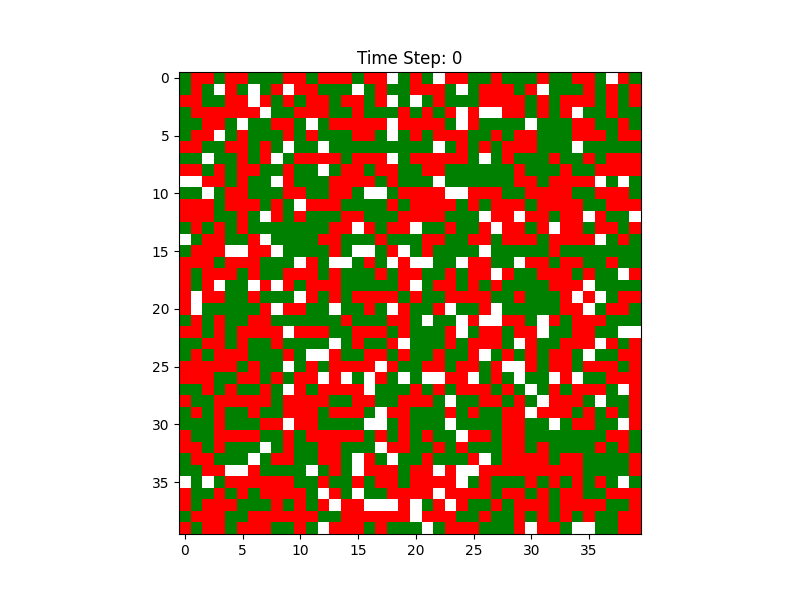
\includegraphics[width=\linewidth]{initial_cluster_w20b20.png}
			\caption{\centering SN w=20, beta=.2}
		\end{subfigure}
		\caption{Initial States}
	\end{figure}
	\begin{figure}[h]
		\centering
		\begin{subfigure}{0.14\textwidth}
			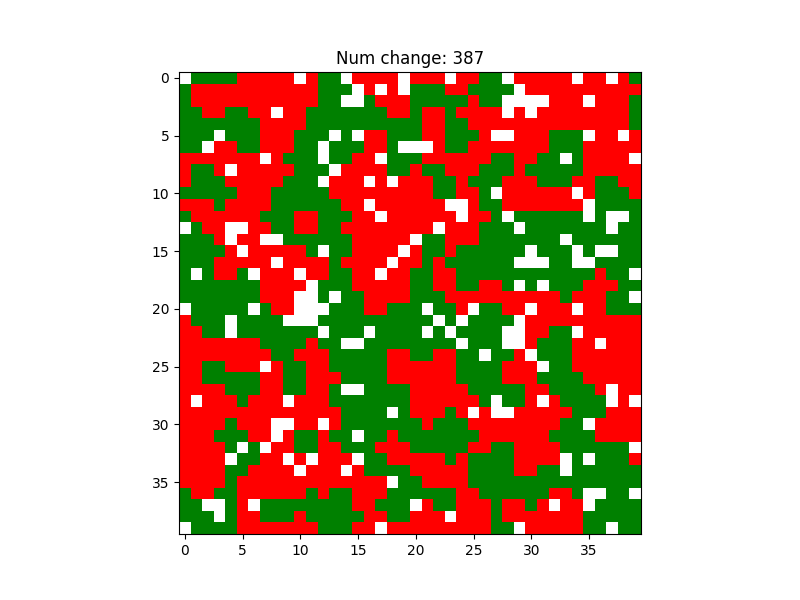
\includegraphics[width=\linewidth]{final_random.png}
			\caption{\centering Random move}
		\end{subfigure}\hfill
		\begin{subfigure}{0.14\textwidth}
			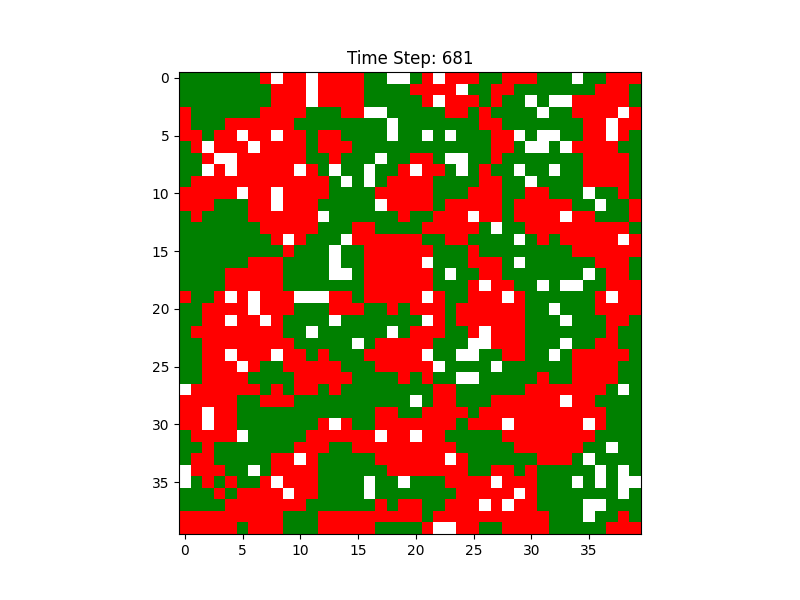
\includegraphics[width=\linewidth]{final_cluster_w5b10.png}
			\caption{\centering SN w=5, beta=.1}
		\end{subfigure}\hfill
		\begin{subfigure}{0.14\textwidth}
			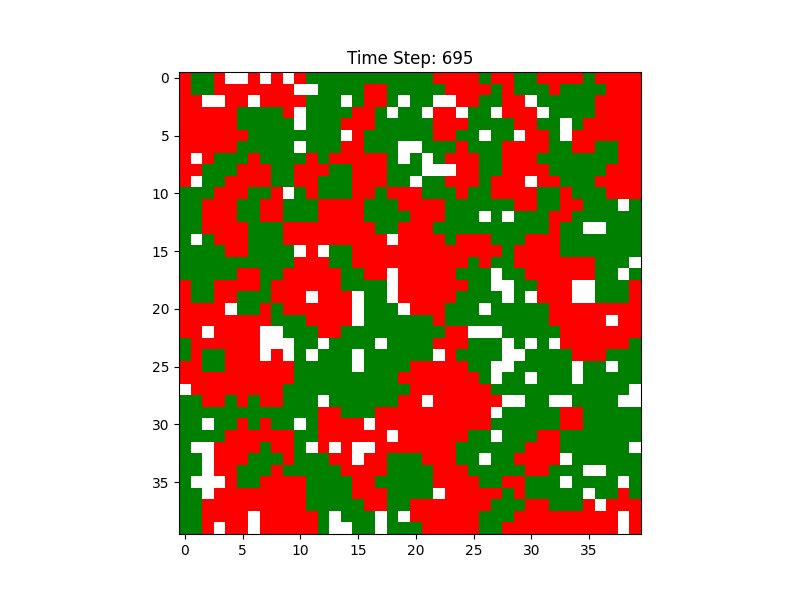
\includegraphics[width=\linewidth]{final_cluster_w10b10.png}
			\caption{\centering SN w=10, beta=.1}
		\end{subfigure}\hfill
		\begin{subfigure}{0.14\textwidth}
			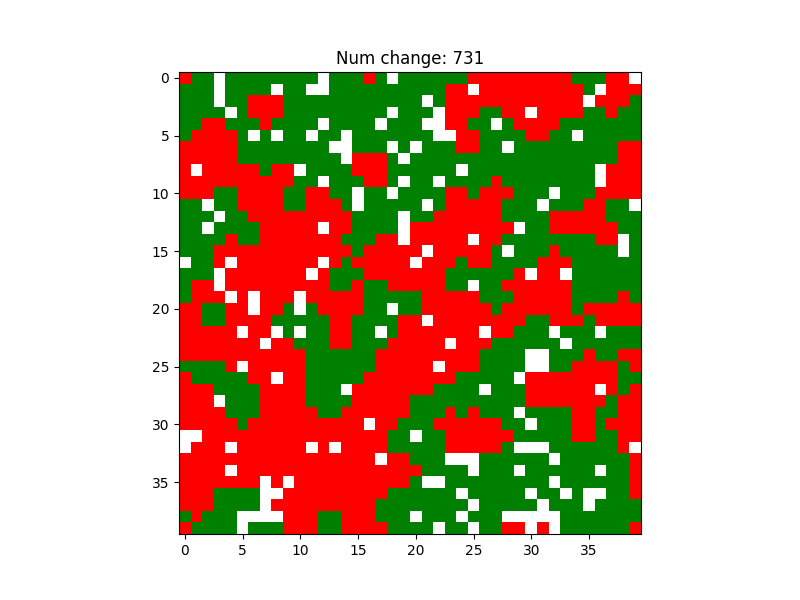
\includegraphics[width=\linewidth]{final_cluster_w20b10.png}
			\caption{\centering SN w=20, beta=.1}
		\end{subfigure}\hfill
		\begin{subfigure}{0.14\textwidth}
			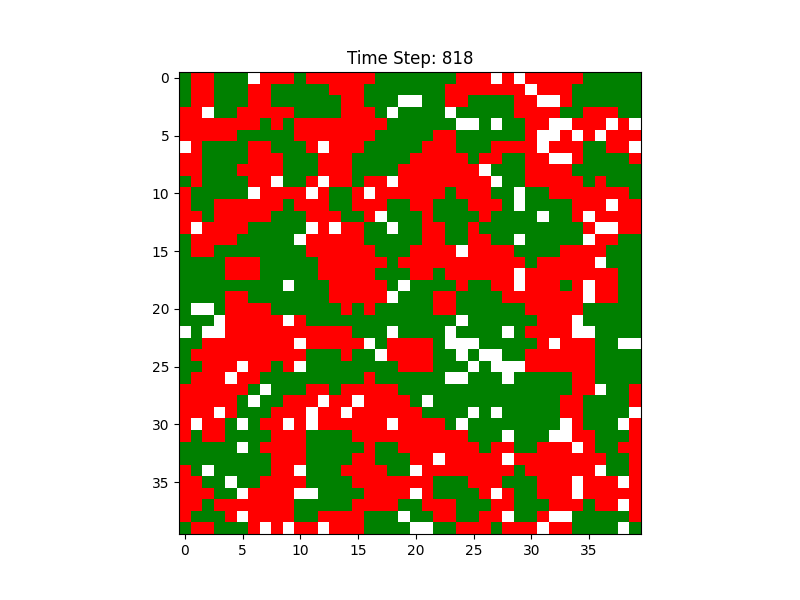
\includegraphics[width=\linewidth]{final_cluster_w5b20.png}
			\caption{\centering SN w=5, beta=.2}
		\end{subfigure}\hfill
		\begin{subfigure}{0.14\textwidth}
			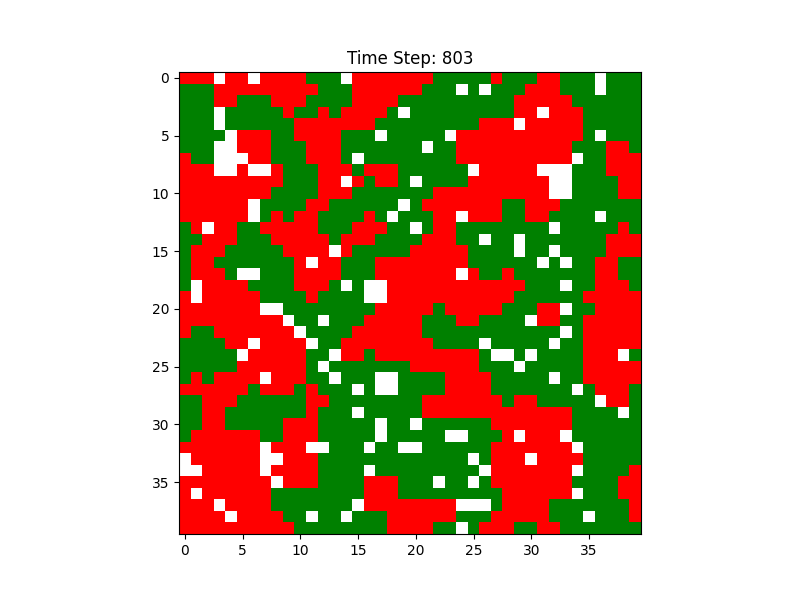
\includegraphics[width=\linewidth]{final_cluster_w10b20.png}
			\caption{\centering SN w=10, beta=.2}
		\end{subfigure}\hfill
		\begin{subfigure}{0.14\textwidth}
			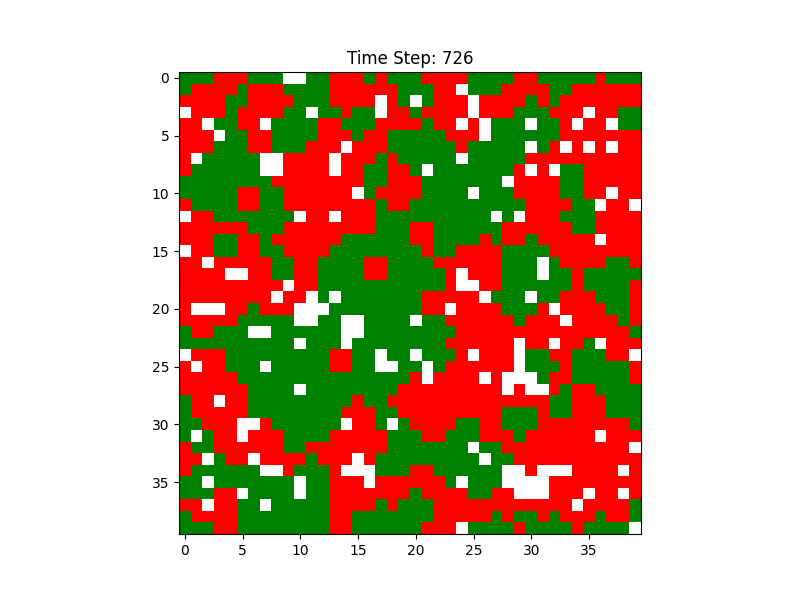
\includegraphics[width=\linewidth]{final_cluster_w20b20.png}
			\caption{\centering SN w=20, beta=.2}
		\end{subfigure}
		\caption{Final states of neighborhood search policies}
	\end{figure}
	\FloatBarrier
	
	\begin{wrapfigure}{l}{.5\textwidth}
		\centering
		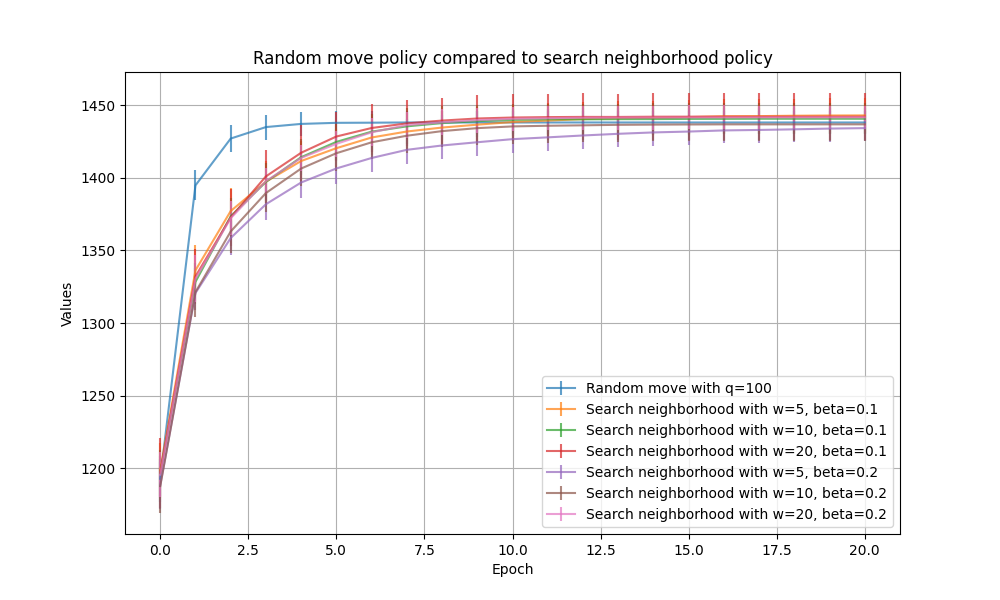
\includegraphics[width=.5\textwidth]{policies02.png}
		\caption{Time series comparison of neighborhood search compared to random move}
	\end{wrapfigure}
	This policy resulted in larger fully connected clusters of Green and Red agents. With the wraparound, the Green smaller clusters are nearly all connected to one another. The Red clusters are also interconnected. Additionally, because of the search only of neighboring spaces, when an empty cluster appears, it often remains open because its spaces are never seen by any of the reporting agents, despite factoring in partial happiness for empty neighboring plots. This method of only talking to a certain degree of separation of neighbors results in a slower convergence to optimal happiness but ends up better than the random move search. Interestingly, the neighborhood search of the smallest separation with less of a chance of talking to mismatched neighbors produced the highest overall average happiness of the automata (ie, talking only to nearby neighbors of the same type). This is perhaps because it makes the agent remain in its own small cluster of like agents instead of hopping between small clusters as could occur with a greater $w$. The standard deviations were all wide enough to include the happiness of the other parameter sets however so there was not a largely significant difference.
	
	\newpage
	
	\subsection{Connor}
	
	
	
	\newpage
	
	\subsection{Josh}
	


\newpage

	
\end{document}